\documentclass[../../main.tex]{subfiles}
\begin{document}

{\bf [解答]}

\paragraph{(1) (イ)}

点$P$が辺上にない場合を考える．この時，半直線$QP$と四角形の交点を$P'$とすると，
$\triangle PQR < \triangle P'QR$となるから，$P'$を新しく点$P$とした方が三角形の面積は大きくなる．点$Q,R$にも同様の議論が適用できるから，面積が最大の三角形では$P, Q, R$ は四角形の辺上にある．

\begin{figure}[htb]
  \centering
  \begin{tikzpicture}[x=1.2cm, y=1.2cm,
    every node/.style={font=\small}]
    \coordinate (D) at (0,0);
    \coordinate (C) at (4,0);
    \coordinate (B) at (5,2);
    \coordinate (A) at (1,2);
    \coordinate (Q) at (2.6,0.4);
    \coordinate (Pprime) at (0.6,1.2);
    \coordinate (P) at ($(Q)!0.55!(Pprime)$);
    \coordinate (R) at (2.8,1.5);
    \fill[red!10] (Pprime)--(Q)--(R)--cycle;
    \fill[blue!20] (P)--(Q)--(R)--cycle;
    \draw[line width=1.2pt, blue!85!black] (D)--(C)--(B)--(A)--cycle;
    \draw[thick, blue!85!black] (P)--(Q)--(R)--cycle;
    \draw[dashed, line width=1.1pt, red!75!black] (P)--(Pprime);
    \draw[dashed, red!75!black] (Pprime)--(R);
    \node[circle, fill, inner sep=1.2pt] at (D) {}; \node[below left=2pt] at (D) {$D$};
    \node[circle, fill, inner sep=1.2pt] at (C) {}; \node[below right=2pt] at (C) {$C$};
    \node[circle, fill, inner sep=1.2pt] at (B) {}; \node[above right=2pt] at (B) {$B$};
    \node[circle, fill, inner sep=1.2pt] at (A) {}; \node[above left=2pt] at (A) {$A$};
    \node[circle, fill, inner sep=1.3pt] at (P) {}; \node[below left=1pt] at (P) {$P$};
    \node[circle, fill, inner sep=1.3pt] at (Q) {}; \node[below=2pt] at (Q) {$Q$};
    \node[circle, fill, inner sep=1.3pt] at (R) {}; \node[above=2pt] at (R) {$R$};
    \node[circle, fill=red!75!black, inner sep=1.5pt] at (Pprime) {};
    \node[left=2pt, red!75!black] at (Pprime) {$P'$};
  \end{tikzpicture}
  \caption{内点 $P$ を半直線 $QP$ と辺 $AD$ の交点 $P'$ へ移したときの面積比較}
  \label{fig:1966_2_move_to_edge}
\end{figure}

\paragraph{(1) (ロ)}

(イ)から，各点が平行四辺形の辺上にある場合のみを考えれば良い．
$P, Q, R$ のうち2点が同一辺上にある時は，その2点を頂点にした時が面積最大であり，この時の面積は
\begin{align}
  \triangle = \dfrac{\square ABCD}{2} \label{eq:1}
\end{align}
である．

\begin{figure}[htb]
  \centering
  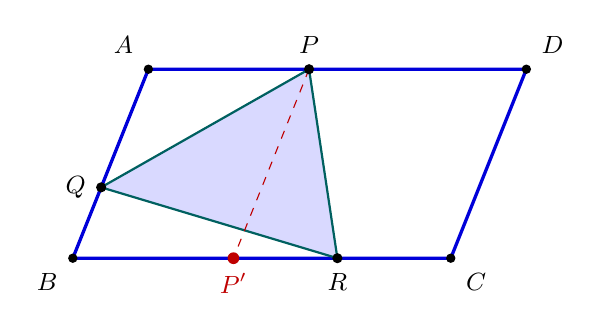
\begin{tikzpicture}[x=1.2cm, y=1.2cm,
    every node/.style={font=\small}]
    \coordinate (B) at (0,0);
    \coordinate (C) at (4,0);
    \coordinate (D) at (4.8,2);
    \coordinate (A) at (0.8,2);
    \coordinate (P) at (2.5,2);
    \coordinate (Pprime) at (1.7,0);
    \coordinate (Q) at (0.3,0.75);
    \coordinate (R) at (2.8,0);
    \fill[blue!15] (P)--(Q)--(R)--cycle;
    \draw[line width=1.2pt, blue!85!black] (B)--(C)--(D)--(A)--cycle;
    \draw[thick, teal!75!black] (P)--(Q)--(R)--cycle;
    \draw[dashed, red!75!black] (P)--(Pprime);
    \node[circle, fill, inner sep=1.2pt] at (A) {}; \node[above left=2pt] at (A) {$A$};
    \node[circle, fill, inner sep=1.2pt] at (B) {}; \node[below left=2pt] at (B) {$B$};
    \node[circle, fill, inner sep=1.2pt] at (C) {}; \node[below right=2pt] at (C) {$C$};
    \node[circle, fill, inner sep=1.2pt] at (D) {}; \node[above right=2pt] at (D) {$D$};
    \node[circle, fill, inner sep=1.3pt] at (P) {}; \node[above=2pt] at (P) {$P$};
    \node[circle, fill, inner sep=1.3pt] at (Q) {}; \node[left=2pt] at (Q) {$Q$};
    \node[circle, fill, inner sep=1.3pt] at (R) {}; \node[below=2pt] at (R) {$R$};
    \node[circle, fill=red!75!black, inner sep=1.5pt] at (Pprime) {}; \node[red!75!black, below=2pt] at (Pprime) {$P'$};
  \end{tikzpicture}
  \caption{$PP'\parallel AB$ としたときの $P,Q,R$ の配置}
  \label{fig:1966_2_parallel_construction}
\end{figure}

次に3点とも異なる辺上にある時を考えよう．
対称性から図のように$P$を辺$AD$上，$Q$を辺$AB$上，$R$を辺$BC$上におく．
$P$ を通り $AB$ に平行な直線と $BC$ の交点を $P'$ とする．まず $P, R$ を固定して考える．

\begin{figure}[htb]
  \centering
  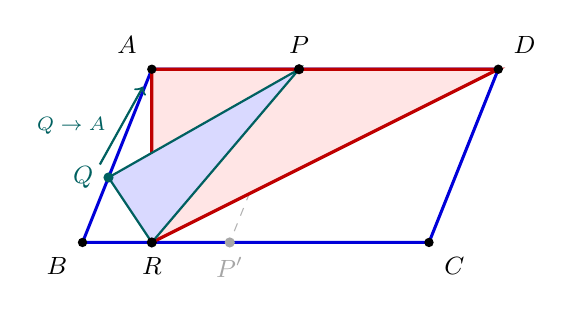
\begin{tikzpicture}[x=1.1cm, y=1.1cm,
    every node/.style={font=\small}]
    \coordinate (B) at (0,0);
    \coordinate (C) at (4,0);
    \coordinate (D) at (4.8,2);
    \coordinate (A) at (0.8,2);
    \coordinate (P) at (2.5,2);
    \coordinate (Pprime) at (1.7,0);
    \coordinate (R) at (0.8,0);
    \coordinate (Q) at (0.3,0.75);

    % 平行四辺形
    \draw[line width=1.1pt, blue!85!black] (B)--(C)--(D)--(A)--cycle;
    \draw[dashed, gray!60] (P)--(Pprime);

    % 最大三角形 (Q=A, P=Dのとき)
    \fill[red!10] (D)--(A)--(R)--cycle;
    \draw[line width=1.2pt, red!75!black] (D)--(A)--(R)--cycle;

    % 元の三角形 PQR
    \fill[blue!15] (P)--(Q)--(R)--cycle;
    \draw[thick, teal!75!black] (P)--(Q)--(R)--cycle;
    \draw[->, thick, teal!75!black] (0.2, 0.9) -- (0.7, 1.8) node[midway, left=2pt, font=\scriptsize] {$Q \to A$};

    \node[circle, fill, inner sep=1.2pt] at (A) {}; \node[above left=2pt] at (A) {$A$};
    \node[circle, fill, inner sep=1.2pt] at (B) {}; \node[below left=2pt] at (B) {$B$};
    \node[circle, fill, inner sep=1.2pt] at (C) {}; \node[below right=2pt] at (C) {$C$};
    \node[circle, fill, inner sep=1.2pt] at (D) {}; \node[above right=2pt] at (D) {$D$};
    \node[circle, fill, inner sep=1.3pt] at (P) {}; \node[above=2pt] at (P) {$P$};
    \node[circle, fill=teal!75!black, inner sep=1.3pt] at (Q) {}; \node[left=2pt, teal!75!black] at (Q) {$Q$};
    \node[circle, fill, inner sep=1.3pt] at (R) {}; \node[below=2pt] at (R) {$R$};
    \node[circle, fill=gray!70, inner sep=1.3pt] at (Pprime) {}; \node[below=2pt, gray!70] at (Pprime) {$P'$};
  \end{tikzpicture}
  \caption{$R$ が $BP'$ 上にあるときの面積最大化（$Q\to A, P\to D$）}
  \label{fig:1966_2_case1}
\end{figure}

$PR$ を底辺とみて，$Q=A$ の時 $\triangle PQR$ は最大である．
このもとで $P$ をうごかすと，$QP$を底辺と見て $P=D$ の時 $\triangle PQR$ は最大値 $\dfrac{1}{2}\square ABCD$ をとる．

\subparagraph{$2^\circ$ $R$ が $P'C$ 上にある時}

\begin{figure}[htb]
  \centering
  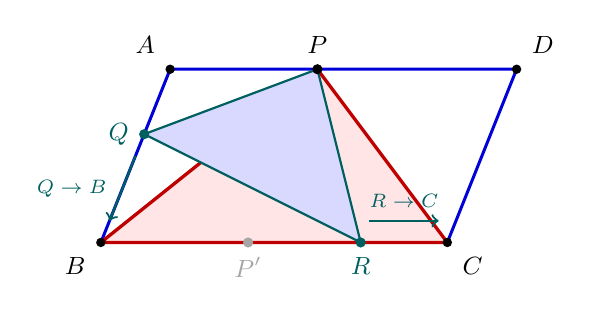
\begin{tikzpicture}[x=1.1cm, y=1.1cm,
    every node/.style={font=\small}]
    \coordinate (B) at (0,0);
    \coordinate (C) at (4,0);
    \coordinate (D) at (4.8,2);
    \coordinate (A) at (0.8,2);
    \coordinate (P) at (2.5,2);
    \coordinate (Pprime) at (1.7,0);
    \coordinate (R) at (3.0,0);
    \coordinate (Q) at (0.5,1.25);

    % 平行四辺形
    \draw[line width=1.1pt, blue!85!black] (B)--(C)--(D)--(A)--cycle;
    \draw[dashed, gray!60] (P)--(Pprime);

    % 最大三角形 (Q=B, R=Cのとき)
    \fill[red!10] (P)--(B)--(C)--cycle;
    \draw[line width=1.2pt, red!75!black] (P)--(B)--(C)--cycle;

    % 元の三角形 PQR
    \fill[blue!15] (P)--(Q)--(R)--cycle;
    \draw[thick, teal!75!black] (P)--(Q)--(R)--cycle;
    \draw[->, thick, teal!75!black] (0.4, 1.0) -- (0.1, 0.25) node[midway, left=2pt, font=\scriptsize] {$Q \to B$};
    \draw[->, thick, teal!75!black] (3.1, 0.25) -- (3.9, 0.25) node[midway, above=1pt, font=\scriptsize] {$R \to C$};

    \node[circle, fill, inner sep=1.2pt] at (A) {}; \node[above left=2pt] at (A) {$A$};
    \node[circle, fill, inner sep=1.2pt] at (B) {}; \node[below left=2pt] at (B) {$B$};
    \node[circle, fill, inner sep=1.2pt] at (C) {}; \node[below right=2pt] at (C) {$C$};
    \node[circle, fill, inner sep=1.2pt] at (D) {}; \node[above right=2pt] at (D) {$D$};
    \node[circle, fill, inner sep=1.3pt] at (P) {}; \node[above=2pt] at (P) {$P$};
    \node[circle, fill=teal!75!black, inner sep=1.3pt] at (Q) {}; \node[left=2pt, teal!75!black] at (Q) {$Q$};
    \node[circle, fill=teal!75!black, inner sep=1.3pt] at (R) {}; \node[below=2pt, teal!75!black] at (R) {$R$};
    \node[circle, fill=gray!70, inner sep=1.3pt] at (Pprime) {}; \node[below=2pt, gray!70] at (Pprime) {$P'$};
  \end{tikzpicture}
  \caption{$R$ が $P'C$ 上にあるときの面積最大化（$Q\to B, R\to C$）}
  \label{fig:1966_2_case2}
\end{figure}

$PR$を底辺と見て$Q=B$の時に $\triangle PQR$ は最大である．
このもとで $R$ を動かすと，$RB$を底辺と見て $R=C$の時に $\triangle PQR$は最大値 $\dfrac{1}{2}\square ABCD$ をとる．
\casesend

以上から，いずれの場合の最大値も$\dfrac{1}{2}\square ABCD$である．
それぞれの場合で$\triangle PQR$の一つの辺は$\square ABCD$の辺に一致するから題意は示された．

\paragraph{(2)}

(i)から，面積 $S$ の平行四辺形の内に入る三角形の最大面積が $\dfrac{1}{2}S$ だから，$S < 2$ の時は$\dfrac{1}{2}S < 1$ となり，面積 1 の三角形は入らない．よって題意は示された．

\newpage

\end{document}
